\documentclass[10pt,a4paper]{article}
% Harava user guide. Built with:  pdflatex user_guide.tex  (three times, for the contents)
% The screenshots are in guide_img/ (taken from the running app with the author's own Fieldwatch log of 8 November 2026).
% Same look as the WSPR Logger user guide.
\usepackage[T1]{fontenc}
\usepackage[utf8]{inputenc}
\usepackage{mathptmx}
\usepackage[scaled=.92]{helvet}
\usepackage{courier}
\usepackage{microtype}
\usepackage[a4paper,margin=2.0cm,top=2.3cm,bottom=2.2cm,headsep=0.5cm]{geometry}
\usepackage{graphicx}
\usepackage{xcolor}
\usepackage{booktabs}
\usepackage{tabularx}
\usepackage{array}
\usepackage{enumitem}
\usepackage{caption}
\usepackage{float}
\usepackage{fancyhdr}
\usepackage{textcomp}
\usepackage{amsmath}
\usepackage{amssymb}
\usepackage{tikz}
\usetikzlibrary{arrows.meta,positioning}
\usepackage[hidelinks]{hyperref}

\definecolor{accent}{HTML}{0369A1}
\definecolor{boxbg}{HTML}{F1F6FA}
\definecolor{warnbg}{HTML}{FFF7E8}
\definecolor{warn}{HTML}{B45309}
\captionsetup{font=small,labelfont=bf,labelsep=period,justification=justified,singlelinecheck=false}
\setlist{itemsep=1.5pt,topsep=3pt,parsep=0pt}
\setlength{\parindent}{0pt}
\setlength{\parskip}{4.5pt plus 1pt}
\renewcommand{\arraystretch}{1.15}
\setcounter{tocdepth}{2}
\pagestyle{fancy}
\fancyhf{}
\fancyhead[L]{\small\itshape Harava --- what your phone heard, raked together}
\fancyhead[R]{\small\itshape User guide, version 1.2 --- November 2026}
\fancyfoot[C]{\small\thepage}
\renewcommand{\headrulewidth}{0.3pt}
\hypersetup{pdftitle={Harava - User guide},pdfauthor={Otso Laakso, OH2GAX}}

\newcommand{\dBm}{\,dBm}
\newcommand{\ui}[1]{\textsf{\small #1}}            % a word on the screen: button, switch, card title
\newcommand{\lead}[1]{\textbf{#1}\enspace}           % run-in paragraph head
\newcommand{\fig}[3]{\begin{figure}[H]\centering\includegraphics[width=#2\textwidth]{guide_img/#1}\caption{#3}\end{figure}}
\newcommand{\figpair}[5]{\begin{figure}[H]\centering
  \begin{minipage}[t]{0.485\textwidth}\centering\includegraphics[width=\textwidth]{guide_img/#1}\end{minipage}\hfill
  \begin{minipage}[t]{0.485\textwidth}\centering\includegraphics[width=\textwidth]{guide_img/#2}\end{minipage}
  \caption{#5}\label{#3}\end{figure}}
\newcommand{\infobox}[2]{\par\smallskip\noindent\fcolorbox{accent!60}{boxbg}{\begin{minipage}{\dimexpr\textwidth-2\fboxsep-2\fboxrule\relax}\small
  \textbf{#1}\enspace #2\end{minipage}}\par\smallskip}
\newcommand{\warnbox}[2]{\par\smallskip\noindent\fcolorbox{warn!60}{warnbg}{\begin{minipage}{\dimexpr\textwidth-2\fboxsep-2\fboxrule\relax}\small
  \textbf{#1}\enspace #2\end{minipage}}\par\smallskip}

\begin{document}
\thispagestyle{plain}
\begin{center}
{\small Harava project \quad$\cdot$\quad User guide, version 1.2 \quad$\cdot$\quad 9 November 2026}\par\vspace{10pt}
{\LARGE\bfseries Harava}\par\vspace{5pt}
{\large\bfseries How to collect with Fieldwatch and read what your phone heard:\\ import, map, devices, layers and the classroom phone check}\par\vspace{8pt}
{\normalsize Otso Laakso (OH2GAX)}\par
{\small \emph{harava} is Finnish for \emph{rake} \quad$\cdot$\quad on your own computer or at \texttt{harava.oh2gax.org}}
\end{center}
\vspace{2pt}

\infobox{In short.}{The Fieldwatch app on an Android phone listens to the Wi-Fi access points and Bluetooth~LE gadgets around you: routers, phones, earbuds, cars, trackers such as AirTags, smart glasses, sensors. It only listens; it never connects to anything. Harava takes what Fieldwatch wrote down and lets you look through it on your computer:
\begin{itemize}[leftmargin=1.2em]
\item \textbf{what was around you and where} --- the map with your path and one pin per radio, a timeline of the day, and a detail card for every radio (Section~\ref{sec:map});
\item \textbf{what kind of radios they were} --- device layers such as Glasses \& VR, Trackers, Vehicles and Phones, each with its own switch (Section~\ref{sec:layers});
\item \textbf{every radio in one list} --- the Devices page with filters, tags and CSV export, and \emph{My devices}, which hides your own router, PC and phone (Sections~\ref{sec:devices}--\ref{sec:mine});
\item \textbf{are all phones in the box?} --- the Phone check for a classroom (Section~\ref{sec:phone}).
\end{itemize}
Section~\ref{sec:collect} tells how to collect with Fieldwatch so that nothing is missed (use \emph{both} the log and a Sit). Section~\ref{sec:reading} explains what the data can and cannot tell, and Section~\ref{sec:quick} is a one-page quick reference. On a phone, open \texttt{/app} (for example \texttt{harava.oh2gax.org/app}): the \emph{Harava Mobile app} shows the same data one view at a time and uploads exports straight from the phone; it has its own guide under \ui{User guides}.}

\infobox{About the figures.}{All screenshots are from Harava with the author's own Fieldwatch log of 8 November 2026: a day at home with two short car trips. They were taken in the light theme, with \ui{Mask addresses} on (Section~\ref{sec:mask}: the second half of every address and all Wi-Fi names are hidden) and \emph{without the map background}, so the map shows only the path and the pins on a plain grey surface. On your screen the map has streets under them. The numbers on your screen will be different.}

\tableofcontents
\bigskip

% ─────────────────────────────────────────────────────────────────────
\section{Fieldwatch and Harava in a nutshell}\label{sec:nutshell}

\subsection{What Fieldwatch hears}
Every Wi-Fi access point sends a short \emph{beacon} about ten times a second, with its address (BSSID) and usually its network name (SSID). Every Bluetooth~LE gadget that wants to be found sends \emph{advertisements}: its address, sometimes a name, a company number and a few bytes of data. Fieldwatch on your phone picks these up and writes down, for each one, \emph{what} was heard (address, name, signal strength, the raw bytes) and \emph{where your phone was} at that moment (GPS).

\lead{Signatures.} Fieldwatch compares every radio with its catalog of about 260 \emph{signatures}: patterns in the address, the name, the company number or the data that point to a kind of device --- \emph{Apple AirTags}, \emph{Ray-Ban / Meta glasses}, \emph{Tesla}, \emph{Flock Safety Cameras}, \emph{Ruuvi}, and so on. A signature is a pattern match, not an identity: it says ``this looks like an AirTag'', not whose AirTag it is.

\lead{Random addresses.} Phones, PCs and earbuds change their Bluetooth address every few minutes to protect their owners' privacy. One phone can therefore appear as many radios during a day. Such addresses carry the flag \texttt{RAND}.

\subsection{The log and the Sit}\label{sec:logsit}
Fieldwatch keeps two different records, and Harava reads both:

\begin{table}[H]\small\centering
\begin{tabularx}{\textwidth}{>{\bfseries}p{2.1cm}XX}
\toprule
 & \textbf{Log} (Reports $\rightarrow$ Log export) & \textbf{Sit} (Reports $\rightarrow$ Start sit \dots\ End sit, then Sit export)\\
\midrule
What & hear by hear: time, signal, raw data, vendor, position & one row per radio for the whole sit: first and last heard, number of hits, weakest and strongest signal, signatures, \emph{Mine}\\
Gaps & a row the first time a radio is heard, then every 25th hear, \textbf{at most 16 rows per scan}; a radio heard briefly in a crowded place can be missed & keeps \textbf{every} radio, up to 6000\\
Needs & \ui{Write to disk} on & nothing extra\\
Gives Harava & the timeline, the path, the signal chart, the Phone check & the complete list, and what the log missed\\
\bottomrule
\end{tabularx}
\caption{The two records of Fieldwatch. Use both.}
\end{table}

\begin{figure}[H]\centering
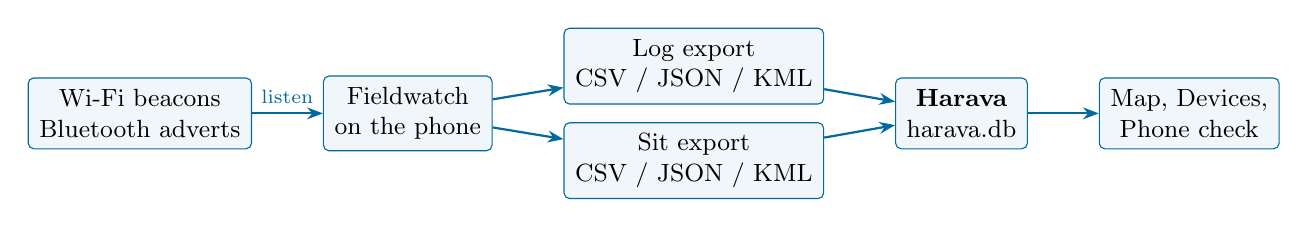
\begin{tikzpicture}[node distance=7mm and 9mm, box/.style={draw=accent,rounded corners=2pt,fill=boxbg,align=center,font=\small,inner sep=4pt,minimum height=9mm}, arr/.style={-{Stealth[length=2mm]},accent,thick}]
\node[box] (radio) {Wi-Fi beacons\\Bluetooth adverts};
\node[box,right=of radio] (fw) {Fieldwatch\\on the phone};
\node[box,right=of fw,yshift=6mm] (log) {Log export\\CSV / JSON / KML};
\node[box,right=of fw,yshift=-6mm] (sit) {Sit export\\CSV / JSON / KML};
\node[box,right=of log,yshift=-6mm] (har) {\textbf{Harava}\\harava.db};
\node[box,right=of har] (views) {Map, Devices,\\Phone check};
\draw[arr] (radio) -- node[above,font=\scriptsize]{listen} (fw);
\draw[arr] (fw) -- (log); \draw[arr] (fw) -- (sit);
\draw[arr] (log) -- (har); \draw[arr] (sit) -- (har);
\draw[arr] (har) -- (views);
\end{tikzpicture}
\caption{From the air to the screen. Fieldwatch listens and exports; you copy the files to your computer; Harava imports them into its own database and shows them.}
\end{figure}

\infobox{Words used in this guide.}{\textbf{Radio}: one Wi-Fi access point or Bluetooth gadget, as one address. \textbf{Hear}: one row of the log (one moment when Fieldwatch wrote the radio down). \textbf{Hear-point}: where \emph{your phone} was at a hear; the place where a radio was heard loudest is its pin on the map. \textbf{RSSI}: received signal strength in dBm; $-30$ is very close, $-60$ in the same room, $-90$ and weaker far away or behind walls. \textbf{Signature}: a Fieldwatch pattern for a kind of device. \textbf{Layer}: one kind of device on the map (Section~\ref{sec:layers}). \textbf{Separated}: a tracker that is away from its owner's phone.}

% ─────────────────────────────────────────────────────────────────────
\section{Collecting data with Fieldwatch}\label{sec:collect}

\lead{Before you go.} In Fieldwatch, turn on \ui{Settings $\rightarrow$ Write to disk} (the log) and \ui{Tag detections with GPS} (positions). Keep the phone charged: listening and GPS use the battery, and the phone gets warm.

\lead{Start a Sit.} \ui{Reports $\rightarrow$ Start sit} names a session: a lesson, a walk, a drive or a whole day. While it runs, the title shows \ui{FIELDWATCH $\cdot$ SIT}. End it with \ui{End sit}. A sit can run all day.

\lead{Export both.} Afterwards export:
\begin{enumerate}[leftmargin=1.5em]
\item \ui{Reports $\rightarrow$ Log export}, format \ui{Log file --- CSV} (JSON lines also works);
\item \ui{Reports $\rightarrow$ Sit export} for the sit, format \ui{Log file --- CSV} (or JSON lines).
\end{enumerate}
Share or save the files and copy them into the \texttt{data} folder of the Harava project on your computer (sub-folders are fine, e.g.\ \texttt{data\textbackslash kml}). KML exports can be imported too, but CSV carries more. The \texttt{data} folder is never committed to git: your exports contain real addresses and your locations.

\warnbox{Why both?}{The Fieldwatch log writes at most 16 rows per scan and writes a radio again only at every 25th hear. In a crowded place --- a classroom, a shopping centre, a busy street --- a gadget that is heard for only a few seconds can be left out of the log altogether. The Sit keeps every radio. With both, Harava shows the timeline from the log \emph{and} marks the radios that only the Sit caught (\ui{sit only}).}

\lead{Fieldwatch's own KML files and Google Earth.} Fieldwatch version 1.1.42 writes hidden Wi-Fi names as invisible zero characters into its KML files, and Google Earth refuses to open them. Harava removes those characters when it imports, so the files load fine.

% ─────────────────────────────────────────────────────────────────────
\section{Installing and starting Harava}\label{sec:start}
Harava is a small program in Python that shows its pages in your web browser. It runs on your own computer, where everything stays with you, or on a server such as \url{https://harava.oh2gax.org}, where you sign in (Section~\ref{sec:signin}). Setting up a server is described in the \emph{Harava Admin and server guide}.
\begin{enumerate}[leftmargin=1.5em]
\item Install Python 3.9 or newer from \url{https://www.python.org/} (on Windows, tick \emph{Add python.exe to PATH}).
\item Double-click \texttt{start\_harava.bat} in the Harava project folder. The first time it installs the one library it needs (Flask).
\item The browser opens at \url{http://127.0.0.1:5057}. Close the black window (or press Ctrl+C in it) to stop Harava.
\end{enumerate}

\lead{The map key.} The map background comes from CARTO. Without a free key it shows an ``API key required'' watermark. Put the key into \texttt{api\_keys.py} (copy \texttt{api\_keys.py.example}) as \texttt{CARTO\_API\_KEY = "\dots"}, exactly as in WSPR Logger. The file never leaves your computer.

\lead{Settings.} Copy \texttt{config.ini.example} to \texttt{config.ini} to change the port, the folder that \ui{Scan folder} reads (\texttt{data}), whether a browser opens at start, and how far apart a radio must be heard to count as \emph{travelled} (500\,m).

\begin{table}[H]\small\centering
\begin{tabularx}{\textwidth}{>{\ttfamily}p{4.1cm}X}
\toprule
\normalfont\textbf{File} & \textbf{What it is}\\
\midrule
start\_harava.bat & starts Harava (Windows); \texttt{python harava.py} does the same\\
harava.py & the program\\
harava.db & your database: all imports, My devices; delete it to start from scratch\\
harava\_users.db & the users and their permissions (only when users exist)\\
api\_keys.py & your CARTO map key (local only)\\
config.ini & your settings (optional)\\
doc/ & this guide, \texttt{whats\_new.md} and \texttt{guides.json}\\
data/ & your Fieldwatch exports; \emph{Scan folder} reads them (not in git)\\
tmp\_files/ & your own working files (not in git)\\
\bottomrule
\end{tabularx}
\caption{The files of Harava.}
\end{table}

% ─────────────────────────────────────────────────────────────────────
\section{Signing in and permissions}\label{sec:signin}
\begin{minipage}[c]{0.36\textwidth}\centering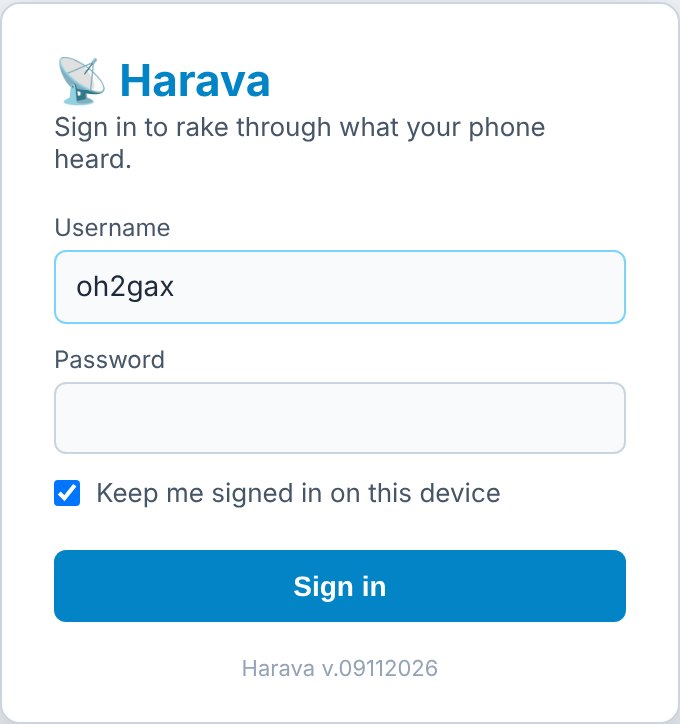
\includegraphics[width=\textwidth]{guide_img/a_login.jpg}\end{minipage}\hfill
\begin{minipage}[c]{0.60\textwidth}
On your own computer Harava opens at once. On a server, and on any Harava where an admin has added users, it first shows a sign-in page. Type your username and password; \ui{Keep me signed in on this device} remembers you for 30 days. The menu then shows your name and permission under the title, and the power button next to the theme button signs you out.

After five wrong passwords from the same place, Harava waits 15 minutes before it lets anyone try again from there.
\end{minipage}

\begin{table}[H]\small\centering
\begin{tabularx}{\textwidth}{>{\bfseries}p{2.4cm}X}
\toprule
Permission & What you can do\\
\midrule
View only & look at everything: the map, the Devices list, the Phone check, the Identification page and the guides; export CSV\\
Analyze & also change the data: upload and import Fieldwatch exports, \ui{Scan folder}, switch or delete imports, add or remove My devices, \ui{Reload database}\\
Admin & also manage the users on \ui{Maintenance}\\
\bottomrule
\end{tabularx}
\caption{The three permissions. Buttons that need a permission you do not have are not shown.}
\end{table}

\lead{Your first sign-in.} The admin gives you a one-time password. Harava then opens \emph{My account}, where you choose your own password (at least 12 characters). Later you find \emph{My account} by clicking your name in the menu; changing the password there signs out your other devices.

\lead{Forgotten password.} Ask the admin for a new one-time password (\ui{New password} on the Maintenance page). Users, permissions and the Maintenance page are described in the \emph{Admin and server guide}.

% ─────────────────────────────────────────────────────────────────────
\section{The page at a glance}\label{sec:glance}
\fig{g_full.jpg}{1.0}{Harava with the log of 8 November 2026. Left: the menu. Top: the timeline of the day. Middle: your path (dashed line) and the pins of the radios. Right: the categories of the radios heard.}

The menu on the left, from the top:
\begin{itemize}[leftmargin=1.2em]
\item \textbf{Harava} with the number of days and files, your name and permission (when you are signed in), and \ui{What's new} with the version badge. The badge turns amber when there are notes you have not read. It opens one window with three tabs: \ui{What's new}, \ui{User guides} (this guide) and \ui{About}. The sun / moon button switches between Auto, Dark and Light; the power button signs you out; \ui{$\blacktriangleleft$} hides the menu (a \ui{$\blacktriangleright$} handle on the left edge brings it back).
\item \textbf{Pages}: \ui{Map}, \ui{Devices}, \ui{Phone check}, \ui{Identification}, \ui{Imports}, and \ui{Maintenance} for admins.
\item \textbf{Day} and an optional \textbf{From--to} time; \ui{$\blacktriangleleft$ $\blacktriangleright$} step a day. \ui{All days} shows everything.
\item \textbf{Filter}: search, Wi-Fi / Bluetooth, minimum RSSI and five switches (Section~\ref{sec:filters}).
\item \textbf{Device layers}: one switch per kind of radio (Section~\ref{sec:layers}).
\item \textbf{Map layers}: the phone path, the timeline graph, the categories card, \ui{Spread stacked pins} and \ui{Mask addresses} (Section~\ref{sec:mask}).
\item \textbf{Shown now}: devices, hears, Wi-Fi, Bluetooth, trackers and travelled radios after the filters.
\end{itemize}

\fig{g_whatsnew.jpg}{0.5}{\ui{What's new} opens one window with three tabs: the notes of each version, the user guides (PDF) and About.}

% ─────────────────────────────────────────────────────────────────────
\section{Importing}\label{sec:import}
\fig{g_imports.jpg}{1.0}{The Imports page. The log of 8 November is on; Fieldwatch's own KML of the same day was switched off automatically, because it repeats the same radios.}

\lead{Two ways in.} Drop files on the dashed box (or \ui{choose files}), or press \ui{Scan folder}. It reads every new \texttt{.csv}, \texttt{.jsonl} and \texttt{.kml} in the \texttt{data} folder, sub-folders included. A file that is already imported is skipped, even under another name.

\lead{What Harava recognises.} Fieldwatch log CSV and JSON lines, Sit export CSV and JSON lines (type \ui{SIT}), and KML from both (the Sit KML also brings your walking path).

\lead{Clean counts by themselves.} When files cover the same time:
\begin{itemize}[leftmargin=1.2em]
\item a \textbf{KML} is switched off when a log or Sit of the same time is already there (a KML repeats the same radios);
\item a \textbf{newer export of the same sit} replaces the older one, which is switched off;
\item a \textbf{log and a Sit} of the same time stay on together: they complement each other.
\end{itemize}
The \ui{Use} switch turns a file on or off by hand; \ui{Delete} removes it from the database (the file itself is not touched). Radios marked \emph{Mine} in a Sit export are added to My devices (Section~\ref{sec:mine}).

% ─────────────────────────────────────────────────────────────────────
\section{The map}\label{sec:map}

\subsection{Path and pins}
The \textbf{dashed line} is your path: where your phone was, in time order, from the GPS positions of the hears. A gap of more than 30 minutes without positions breaks the line.

Each radio has \textbf{one pin}, at the place where your phone heard it \emph{loudest}. That is a good guess of where the radio was, but only a guess: the pin is always on your path, never off it.
\begin{itemize}[leftmargin=1.2em]
\item \textbf{filled} pin = Bluetooth, \textbf{ring} = Wi-Fi, \textbf{bigger} = louder;
\item the colour is the device layer (Section~\ref{sec:layers});
\item watch-list radios (glasses, trackers, surveillance, police, drones, hacking tools) get a round \textbf{icon pin} on top of the others; a tracker that is \emph{separated} from its owner \textbf{pulses red};
\item where many radios share one spot (at home, most do), \ui{Spread stacked pins} lays them out in a small sunflower so that each one can be clicked. Zoom in to see them.
\end{itemize}
Hover over a pin for its name, layer, signal and hears; click it for its details.

\fig{g_trackers.jpg}{0.9}{Only the \emph{Tracker} layer, zoomed in at home. Each tag icon is one tracker address heard during the day. All were weak and heard once or twice --- neighbours' tags and passers-by, nothing that followed the phone.}

\subsection{The timeline}\label{sec:timeline}
\fig{g_timeline.jpg}{0.95}{Hears per 10 minutes: Wi-Fi (blue) and Bluetooth (green) bars, and the number of new radios (line, right scale). The busy peaks around 08:00--11:00 are at home; the drives show as short bursts of many new radios.}
The bars count the hears in each 10-minute step (each hour or day when you look at a longer period); the line counts the radios heard for the first time in that step. \textbf{Click a bar} to look at just those 10 minutes; clear the From--to times to see the whole day again.

\lead{Show one kind of device.} The \ui{Show} selector in the title limits the graph to one layer, for example \ui{Glasses \& VR only} or \ui{Tracker only}; the number in brackets is how many such radios the day has. \emph{none heard in this range} means there were none. The selector changes only the graph, not the map.

\fig{g_timeline_trk.jpg}{0.95}{The same day with \ui{Tracker only}: when the trackers were heard.}

\subsection{The selected radio}
\begin{figure}[H]\centering
\begin{minipage}[c]{0.63\textwidth}\centering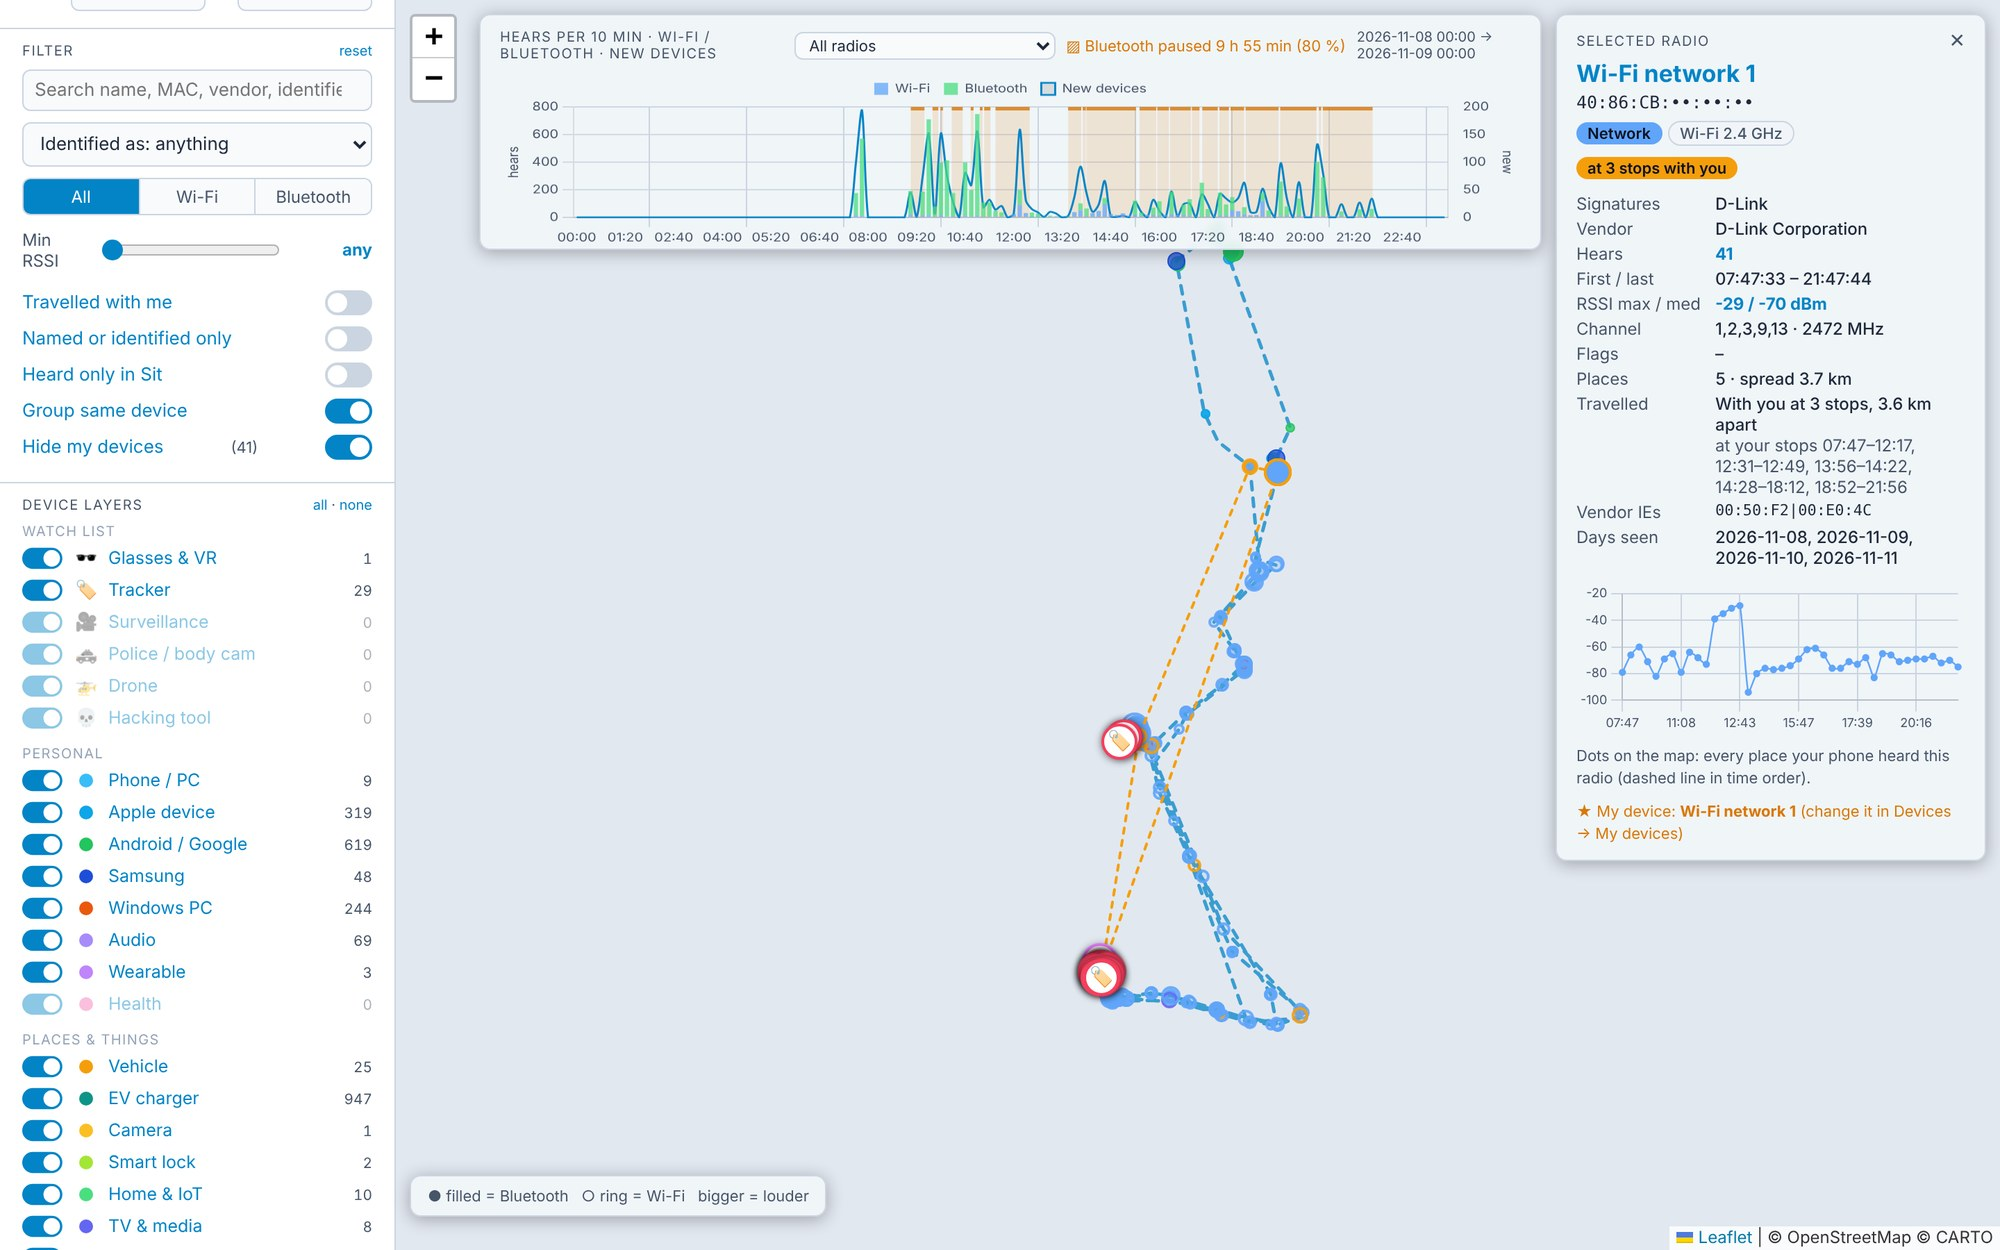
\includegraphics[width=\textwidth]{guide_img/g_selected.jpg}\end{minipage}\hfill
\begin{minipage}[c]{0.34\textwidth}\centering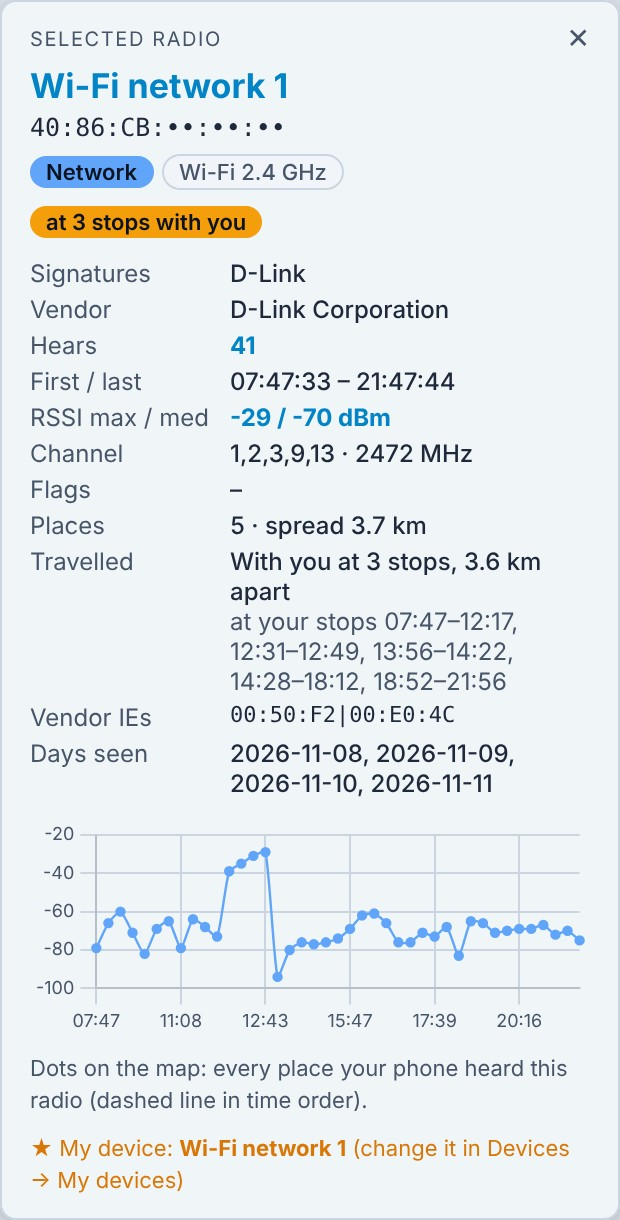
\includegraphics[width=\textwidth]{guide_img/g_detail.jpg}\end{minipage}
\caption{The D-Link 4G router selected (left), and its panel enlarged (right). Its hear-points are joined by the amber dashed line: the same address was heard at home and 3.7\,km away, so it \emph{travelled} with the phone. The chart shows its signal over the day: about $-70$\dBm at home and $-29$\dBm at the first stop.}
\end{figure}

Clicking a pin (or a row of the Devices page) opens the \textbf{Selected radio} panel at the top right and draws every place where the radio was heard. Close it with \ui{$\times$}; click any pin to open it again.

\begin{table}[H]\small\centering
\begin{tabularx}{\textwidth}{>{\bfseries}p{2.7cm}X}
\toprule
Field & What it tells\\
\midrule
Name, address & the advertised name and the MAC address; \emph{(hidden network)} for a Wi-Fi without a name\\
Pills & the layer, the radio (Wi-Fi band or Bluetooth LE), and \emph{travelled} with the distance\\
Signatures, vendor & the Fieldwatch signatures that matched, and the maker of the address block\\
Tracker mode & \emph{separated} (away from its owner) or \emph{near owner}, read from the raw data\\
Sensor & a Ruuvi tag's temperature, humidity, pressure and battery\\
Hears & how many times it was written down; with a Sit, also the log rows and the Sit hits\\
First / last & the first and last time heard (in the chosen range)\\
RSSI max / med & the strongest and the typical signal; \emph{Sit RSSI} gives the sit's weakest \dots\ strongest\\
Places, spread & in how many places (about 200\,m apart) and over what distance it was heard\\
Identified as & what Harava's own database says the radio is, with a confidence pill (Section~\ref{sec:ids})\\
Company & the company from the official Bluetooth SIG list\\
Same device & how many addresses the same device used, when Harava can tell\\
Company ID, services, raw & the Bluetooth data, for the curious\\
Days seen & every day in your imports on which this address appears\\
\bottomrule
\end{tabularx}
\caption{The fields of the Selected radio panel.}
\end{table}

Under the chart, \ui{+ Mark as my device} adds the radio to My devices (Section~\ref{sec:mine}). A note tells when the address is random, when the name points to a VR headset, and when only the Sit heard the radio.

% ─────────────────────────────────────────────────────────────────────
\section{Device layers}\label{sec:layers}
\begin{figure}[H]\centering
\begin{minipage}[c]{0.3\textwidth}\centering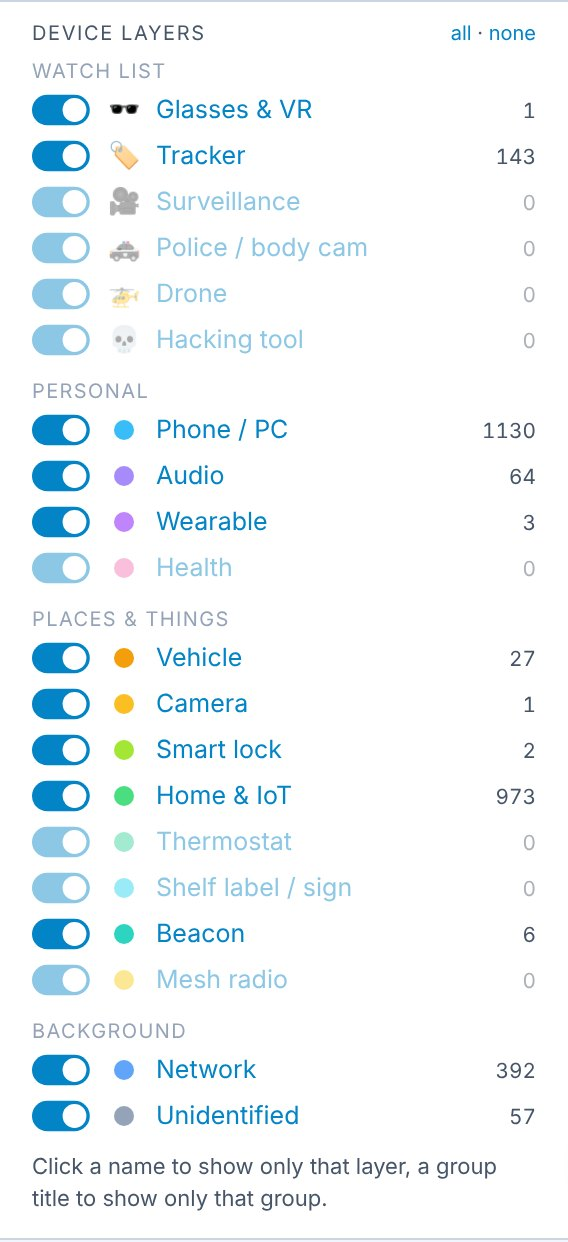
\includegraphics[width=\textwidth]{guide_img/g_layers.jpg}\end{minipage}\hfill
\begin{minipage}[c]{0.66\textwidth}\small
Every kind of device in the Fieldwatch catalog is its own layer with a switch and a count. Layers with nothing in them are dimmed.
\begin{itemize}[leftmargin=1.2em]
\item \textbf{Click a name} to show \emph{only} that layer; click it again to bring all layers back.
\item \textbf{Click a group title} (Watch list, Personal, \dots) to show only that group.
\item \ui{all} / \ui{none} switch every layer at once.
\end{itemize}
Harava remembers your choice. The \emph{Categories} card on the map shows the same counts as bars; a click on a row hides or shows that layer.
\end{minipage}
\caption{The Device layers section of the menu.}
\end{figure}

\begin{table}[H]\small\centering
\begin{tabularx}{\textwidth}{>{\bfseries}p{2.4cm}>{\bfseries}p{2.9cm}X}
\toprule
Group & Layer & Examples from the catalog\\
\midrule
Watch list & Glasses \& VR & Ray-Ban / Meta, Even G1, Snap Spectacles, Vuzix, RayNeo, Brilliant Frame; Meta Quest and other VR headsets\\
(icon pins) & Tracker & Apple AirTags (Find My), Google Find Hub, Samsung SmartTag, Tile, Chipolo, Pebblebee, DULT\\
 & Surveillance & Flock Safety, Axis, Dahua, traffic sensors (BlipTrack, BlueTOAD)\\
 & Police / body cam & Axon, Digital Ally, in-car routers\\
 & Drone & DJI, Autel, Parrot, Remote ID\\
 & Hacking tool & Flipper Zero, Hak5 Pineapple, Pwnagotchi\\
\midrule
Personal & Phone / PC & Apple devices, Google, Microsoft (Windows PCs), Fast Pair, phone hotspots\\
 & Audio, Wearable, Health & earbuds and speakers; watches, rings, pendants; Dexcom, Omron\\
\midrule
Places \& things & Vehicle & Tesla, Audi MMI, BMW, CarPlay, tyre-pressure sensors\\
 & Camera, Smart lock & Arlo, GoPro, Nest; SALTO, Yale, Nuki\\
 & Home \& IoT, Thermostat & Ruuvi, Govee, Amazon, Hue; ecobee, Nest\\
 & Shelf label / sign, Beacon, Mesh radio & electronic shelf labels; iBeacon, Estimote; Meshtastic, goTenna\\
\midrule
Background & Network & Wi-Fi access points and routers\\
 & Unidentified & no signature matched: most random Bluetooth addresses\\
\bottomrule
\end{tabularx}
\caption{The device layers. A radio that matches several signatures goes to the layer highest in this list (a tracker before a phone).}
\end{table}

\infobox{Glasses \& VR.}{Smart glasses and VR headsets share one layer, because Meta uses the same Bluetooth identity for its Ray-Ban glasses and its Quest headsets; Fieldwatch's \emph{Ray-Ban / Meta glasses} signature matches both. When the name says \emph{Quest}, \emph{Oculus}, \emph{Pico}, \emph{Vive} or \emph{Vision Pro}, Harava adds a \textbf{VR?} tag and a note. Glasses usually advertise without a name. On 8 November the only hit was ``Quest 3'', heard once at $-96$\dBm\ when leaving home --- most likely a neighbour's headset.}

% ─────────────────────────────────────────────────────────────────────
\section{Filters}\label{sec:filters}
The filters change the map, the Devices list and the counts at the same time.
\begin{itemize}[leftmargin=1.2em]
\item \textbf{Search} --- part of a name, address, vendor, signature, layer, \emph{Identified as} or company, e.g. \texttt{tesla}, \texttt{40:86}, \texttt{Ruuvi}, \texttt{hue}.
\item \textbf{Identified as} --- only one kind of identified device, grouped by layer (Section~\ref{sec:ids}).
\item \textbf{All / Wi-Fi / Bluetooth}.
\item \textbf{Min RSSI} --- only radios heard at least this loud; $-70$ leaves roughly what was close.
\item \textbf{Travelled with me} --- the same address heard at least 500\,m apart, in at least two places. Your own phone's companions (car, earbuds, power bank) show up here --- and anything that followed you.
\item \textbf{Named or identified only} --- radios with a name or a signature.
\item \textbf{Heard only in Sit} --- radios that only a Sit export has: what the log missed.
\item \textbf{Group same device} --- on by default; addresses that belong to one device are one row (Section~\ref{sec:ids}).
\item \textbf{Hide my devices} --- on by default; the number is how many of your own radios are hidden now.
\end{itemize}
\ui{reset} clears the filters (not the layers).

% ─────────────────────────────────────────────────────────────────────
\section{The Devices page}\label{sec:devices}
\fig{g_devices.jpg}{1.0}{The Devices page, strongest first. \ui{+} in the first column marks a radio as yours; the star box above it holds My devices.}

One row per radio, with the same filters as the map. Click a column title to sort (again for the other way); click a row to see the radio on the map.

\begin{table}[H]\small\centering
\begin{tabularx}{\textwidth}{>{\bfseries}p{2.6cm}X}
\toprule
Column & Meaning\\
\midrule
$\bigstar$ & \ui{+} marks the radio as yours; $\bigstar$ when it already is (shown when \emph{Hide my devices} is off)\\
Category, Radio & the device layer; Wi-Fi or BLE\\
Name & the advertised name, with tags: \emph{N addr.} (one device, many addresses), \emph{travelled}, \emph{separated} (tracker), \emph{VR?}, \emph{sit only}, a Ruuvi temperature\\
Address, Vendor & MAC address; maker of the address block (empty for random addresses)\\
Identified as & Harava's own identification; grey with \textbf{?} is a weak guess\\
Company / vendor & the Bluetooth company, or else the maker of the address block\\
Signatures & every Fieldwatch signature that matched\\
RSSI max, Median & strongest and typical signal in dBm\\
Hears, Ch & how often written down; Wi-Fi channel(s)\\
First, Last, Spread & first and last heard; distance between its hear-points\\
Flags & \texttt{RAND} random address, \texttt{HIDDEN} hidden network\\
\bottomrule
\end{tabularx}
\caption{The columns of the Devices page.}
\end{table}
\ui{Export CSV} saves the list as it is filtered now, for a spreadsheet. The page shows the first 1500 rows; the export has all.

% ─────────────────────────────────────────────────────────────────────
\section{Identification}\label{sec:ids}
Fieldwatch's signatures name only part of what it hears. On 8 November it left 1,782 Bluetooth radios \emph{Unidentified}. Harava has its own identification database on top of the signatures, and it named 1,725 of them (97\,\%).

\fig{g_ids.jpg}{1.0}{The \ui{Identification} page for 8 November: the counts at the top, the patterns that are still unknown, and the rules with how many radios each matched.}

\lead{What it reads.} A Bluetooth radio advertises a few short pieces of data: a company number, service numbers, and data in a known format. Harava compares them with two files in the \texttt{ids} folder:
\begin{itemize}[leftmargin=1.2em]
\item \texttt{bt\_assigned\_numbers.json} --- the official Bluetooth SIG lists: 4,065 company numbers and 819 service numbers. \texttt{python tools/update\_bt\_numbers.py} downloads the newest lists.
\item \texttt{harava\_ids.json} --- Harava's own rules, for example \emph{Bluetooth Mesh device, not set up}, \emph{AirPods}, \emph{iPhone / iPad / Mac}, \emph{Samsung Galaxy phone}, \emph{Windows PC}, \emph{Oral-B toothbrush}. The first rule that matches wins.
\end{itemize}
A radio that Fieldwatch left \emph{Unidentified} moves to the layer the rule gives, e.g.\ \emph{Home \& IoT} for a mesh light. \emph{Identified as} and \emph{Company / vendor} show the result on the Devices page and in the Selected radio panel. A grey name with \textbf{?} is a weak guess: ``some Apple device'' says only who made it.

\lead{One device, many addresses.} Phones, PCs and many smart-home devices change their Bluetooth address every few minutes. Sometimes the data still proves that addresses belong together: a Bluetooth Mesh device sends its own device number in every advert. Harava then puts them in one group. A service number that a maker uses in all its products is not enough on its own (Ruuvi tags, Windows PCs and Galaxy Buds each share one), so such addresses are joined only when they also tell the same name. With \ui{Group same device} on (in Filter), a group is one row with an \textbf{N addr.} tag; its pin is the loudest address, and the hears are added up.

\fig{g_grouped.jpg}{1.0}{\ui{Identified as: EV charging point (DEFA?)} on the Devices page. On 8 November, 957 addresses folded into 23 devices, most of them the charge points of the housing company's car park; one of them used 216 addresses during the day.}

\lead{Charge points.} The housing company's car park has a shared charging system of about 30 charge points. Its chargers advertise as Bluetooth Mesh devices named ``Charge'' that are not set up, and each one changes its address all the time. On 8 November Harava joined 937 such addresses into 22 charge points; most of them were heard only at 12:15, on the way to the car. A nameless address takes the name from the other adverts of the same device, so all its addresses are shown as a charge point. The maker (most likely DEFA) is not confirmed, hence the question mark.

\lead{Only one kind.} The \ui{Identified as} list under the search box shows only one kind of identified device --- for example \emph{Philips Hue lamp}, \emph{Samsung TV} or \emph{Oral-B electric toothbrush}. The list is grouped by device layer, so the \emph{Home \& IoT} group lists everything Harava found on that layer, each with its count after the other filters. Search finds the same texts too: \texttt{hue} finds the Hue lamp.

\lead{Making it better.} The page lists the most common patterns that are still unknown --- the best place to look for the next rule. Edit \texttt{ids/harava\_ids.json} (it starts with a description of every field) and press \ui{Reload database}; Harava does not need a restart. An identification is a pattern match like a signature: a strong hint, not proof.

% ─────────────────────────────────────────────────────────────────────
\section{My devices}\label{sec:mine}
\fig{g_mydevices.jpg}{1.0}{My devices. A rule ``Name is OTSOPC'' hides the 31 addresses the author's PC used during the day. The form at the top was filled by the \ui{+} button of the D-Link router's row; with \ui{Mask addresses} on, Wi-Fi names show as \emph{Wi-Fi network 1, 2 \dots}}

Your own router, PC, phone, earbuds, sensors and car are heard all the time and fill the lists. Mark them once and they disappear from the Devices list, the map and the Phone check while \ui{Hide my devices} is on. Switch it off to see them again, marked $\bigstar$.

\lead{Adding.} Press \ui{+} on a Devices row or \ui{+ Mark as my device} in the Selected radio panel: the form at the top of the Devices page is filled in. Check the label and press \ui{Add}. You can also type a rule yourself.

\lead{Matching.} \emph{Address is} (one exact address), \emph{Address starts with} (e.g.\ a router's 2.4 and 5\,GHz networks, whose addresses differ only at the end), \emph{Name is}, \emph{Name contains}; optionally only Wi-Fi or only Bluetooth. Bluetooth phones, PCs and earbuds change their address, so match them \textbf{by name}; \ui{+} chooses that for them by itself. The column \emph{Matches now} counts the radios a rule catches in the chosen range. Rules apply to every day, also to files imported later.

% ─────────────────────────────────────────────────────────────────────
\section{The Phone check}\label{sec:phone}
\fig{g_phone.jpg}{1.0}{The Phone check over three minutes of the author's home log (not a classroom), after \ui{Auto-calibrate box} with 30 phones expected: the strong group is ``in the box'', one phone is ``in the room'', the rest are weak.}

\lead{The idea.} At the start of a lesson the pupils put their phones into a box next to the teacher's phone, which runs Fieldwatch. The phones in the box are very close to it, so their signals are \emph{strong} and similar. A phone that stays in a pocket or a bag in the same room is heard \emph{more weakly}; phones outside the room are weaker still. The Phone check sorts the phones of a short time window into these three groups.

\lead{Step by step.}
\begin{enumerate}[leftmargin=1.5em]
\item During the lesson, let Fieldwatch run with the log on. Afterwards export the log and import it.
\item Choose the day in the menu. In the Phone check, set \ui{Window start} to a moment when the phones are in the box, and \ui{Window length} to 2--5 minutes.
\item Set \ui{Expected phones}, e.g.\ 30, and press \ui{Auto-calibrate box}. If at least that many phones are heard, the box limit goes just below the 30th strongest; if fewer, it goes into a clear gap (at least 6\,dB) between the strong group and the rest. It never goes below the room limit. You can type the limits yourself (defaults: box $\geq -55$\dBm, room $\geq -80$\dBm).
\item Read the cards and the verdict: \emph{in box}, \emph{in room, not in box}, \emph{weak / outside}. The chart shows the phones by signal strength (green = box, amber = room). The table lists the phones, the ones in the room first.
\end{enumerate}

\lead{What counts as a phone.} Bluetooth radios of Apple, Samsung and Google / Android, without watches, earbuds, TVs and trackers. Two switches add Windows PCs and unidentified random addresses. iPads and Macs advertise like iPhones and are counted too. Your own devices (My devices) never count, so mark the teacher's phone and laptop as yours.

\warnbox{Things to know.}{\textbf{Short window}: phones change their address about every 15 minutes, so a long window can count one phone twice. \textbf{Silent phones}: a phone that is off, in flight mode or with Bluetooth off sends nothing and cannot be heard; a \textbf{metal box} blocks the signal too --- those phones look \emph{missing}, not \emph{in room}. Use a cardboard or plastic box. \textbf{Calibrate once in the real room}, with a few known phones in the box and a few on desks: bodies, desks and walls weaken the signal. \textbf{The log only}: the Phone check does not use Sit exports, because a Sit row spans the whole session. \textbf{Privacy}: the check counts radios; it does not identify pupils. Agree its use with the school, keep the logs only as long as needed, and follow the school's rules and data-protection law.}

% ─────────────────────────────────────────────────────────────────────
\section{Mask addresses}\label{sec:mask}
A Wi-Fi network's name together with its address can be looked up in public Wi-Fi maps, and your own home network points to your home. Before you share a screenshot, switch on \ui{Mask addresses} under \ui{Map layers}. It changes only what is drawn on the screen:
\begin{itemize}[leftmargin=1.2em]
\item every address keeps only its maker part: \texttt{40:86:CB:••:••:••};
\item every Wi-Fi network name --- your own too --- becomes \emph{Wi-Fi network 1, 2 \dots};
\item other people's PC names become \emph{PC 1, 2 \dots}, and personal names such as \emph{Anna's iPhone} become \emph{•••'s iPhone}. Your own Bluetooth devices keep their names.
\end{itemize}
The data, the CSV export and the database are not changed, and \ui{Add} in My devices still saves the full address. Switch it off to see everything again. All screenshots in this guide were taken with it.

% ─────────────────────────────────────────────────────────────────────
\section{Reading the data}\label{sec:reading}

\lead{A pin is where you were.} Fieldwatch knows where \emph{your phone} was, not where the radio was. The pin at the loudest hear is close to the radio only if you passed close to it. A radio heard from your sofa at $-90$\dBm\ may be in the next house.

\lead{Hears are not minutes.} The log writes a radio the first time and then at every 25th hear; it forgets a radio after 15 minutes of silence (3 minutes for anonymous ones) and writes it again as new. A radio with 40 hears was not necessarily around longer than one with 4.

\lead{One gadget, many addresses.} Random Bluetooth addresses change every few minutes; a phone nearby all day can be dozens of ``radios''. Match your own by name (My devices). Wi-Fi access points keep their address.

\lead{Travelled.} The same address heard in two places at least 500\,m apart went with you --- or followed you. On 8 November two radios did: a D-Link 4G router (about $-70$\dBm\ at home, $-29$\dBm\ at the first stop 3.7\,km away, heard as the phone came and went; it fits a router kept in the car) and a device named EF-R3PB2139 (the name fits an EcoFlow River 3 Plus power station). Random addresses rarely travel, because they change, so a travelling \emph{fixed} address is the interesting case.

\lead{Trackers.} An AirTag or other tag \emph{near its owner} is normal: every Apple user carries some. A tag \emph{separated} from its owner and heard in several places along your way, over a long time, deserves a closer look. Fieldwatch and Harava read the mode from the raw data: for Apple Find My a full-key frame means separated; for Google Find Hub and DULT a flag byte tells it. Signals from one tag change address too, so look at the pattern, not at one address.

\lead{Signatures are patterns.} A signature is a hint, not proof: an OUI (maker) match, a name or a data pattern. \emph{Ray-Ban / Meta glasses} also matches Quest headsets; an \emph{Apple Device} may be an iPhone, a Mac or an iPad.

\lead{Ruuvi sensors.} Harava decodes Ruuvi tags (format 5): temperature, humidity, pressure and battery voltage, shown in the detail panel and as a tag in the list. On 8 November one read about $-17$\,\textdegree C (a freezer) with the weakest battery, 2.55\,V.

% ─────────────────────────────────────────────────────────────────────
\section{Questions you can answer}\label{sec:questions}
\begin{itemize}[leftmargin=1.2em]
\item \emph{Were there smart glasses or VR headsets around me today, and when?} --- \ui{Glasses \& VR} only, and \ui{Show: Glasses \& VR only} in the timeline.
\item \emph{Did anything travel with me that is not mine?} --- \ui{Travelled with me} on, \ui{Hide my devices} on.
\item \emph{Is there a separated tracker along my way?} --- \ui{Tracker} only; look for pulsing red pins and \emph{separated} tags.
\item \emph{What did the log miss?} --- import the Sit export too and switch on \ui{Heard only in Sit}.
\item \emph{Which cars, cameras or locks did I pass?} --- the \ui{Vehicle}, \ui{Camera} and \ui{Smart lock} layers.
\item \emph{Are all phones in the box?} --- the Phone check (Section~\ref{sec:phone}).
\item \emph{How cold is the freezer?} --- search \texttt{Ruuvi} and open the tag.
\item \emph{What was around between 12:30 and 12:45?} --- From--to times in the menu, or a click on the timeline.
\end{itemize}

\section{Limitations}\label{sec:limits}
\begin{itemize}[leftmargin=1.2em]
\item Only what Fieldwatch heard: radios that were silent, too far, or behind metal are not there. A phone hears Bluetooth up to some tens of metres and Wi-Fi a little farther.
\item Positions are the phone's positions; GPS indoors can drift by tens of metres, and the first minutes may have no position at all.
\item The log is thinned (16 rows per scan, every 25th hear); without a Sit, brief radios can be missing.
\item Signatures and identifications can be wrong in both directions, and one gadget can look like many; Harava groups addresses only when the data proves they belong together.
\item A Sit export has no hear-by-hear times: Harava draws the timeline and the path from the log.
\item The Phone check is an indicator for a teacher, not proof about a pupil.
\end{itemize}

% ─────────────────────────────────────────────────────────────────────
\section{Quick reference}\label{sec:quick}
\begin{table}[H]\small\centering
\begin{tabularx}{\textwidth}{>{\bfseries}p{4.2cm}X}
\toprule
I want to \dots & Do this\\
\midrule
start Harava & double-click \texttt{start\_harava.bat}; open \url{http://127.0.0.1:5057}\\
collect without gaps & Fieldwatch: \ui{Write to disk} on + \ui{Start sit}; export Log CSV and Sit CSV\\
bring in new files & copy them into \texttt{data}, \ui{Imports $\rightarrow$ Scan folder}\\
see one day / an hour & \ui{Day}, \ui{From--to}, or click a timeline bar\\
see only one kind of device & click its name under \ui{Device layers} (again for all)\\
graph only glasses & timeline \ui{Show $\rightarrow$ Glasses \& VR only}\\
look at one radio & click its pin or its row; \ui{$\times$} closes the panel\\
hide my own devices & \ui{+} on the row $\rightarrow$ \ui{Add}; \ui{Hide my devices} on\\
find what followed me & \ui{Travelled with me} on\\
find what the log missed & import the Sit export, \ui{Heard only in Sit} on\\
see what Harava identified & \ui{Identification}; edit \texttt{ids/harava\_ids.json}, \ui{Reload database}\\
see one row per device & \ui{Group same device} on\\
see only Hue lamps & \ui{Identified as $\rightarrow$ Philips Hue lamp}\\
share a screenshot & \ui{Mask addresses} on (Map layers)\\
change my password & click your name in the menu (\emph{My account})\\
check the phone box & \ui{Phone check}: window start, 3 min, expected, \ui{Auto-calibrate box}\\
take the list to Excel & \ui{Devices $\rightarrow$ Export CSV}\\
remove a wrong file & \ui{Imports}: switch off or \ui{Delete}\\
see what is new & \ui{What's new} under the name\\
remove the map watermark & CARTO key in \texttt{api\_keys.py}\\
start from scratch & stop Harava, delete \texttt{harava.db}\\
\bottomrule
\end{tabularx}
\caption{Quick reference.}
\end{table}

\vfill
{\small\textit{Harava reads the logs of Fieldwatch by Off Grid Pete (\url{https://github.com/OffGridPete/Fieldwatch}); its device layers come from the Fieldwatch signature catalog (MIT licence). Harava itself is not part of Fieldwatch. Leaflet (BSD-2) and Chart.js (MIT) are bundled; the map background is \copyright~OpenStreetMap contributors \copyright~CARTO.}}

\end{document}
